\begin{center}
    \addcontentsline{toc}{section}{Сравнительный анализ существующих алгоритмов и реализаций}
    \section*{СРАВНИТЕЛЬНЫЙ АНАЛИЗ СУЩЕСТВУЮЩИХ АЛГОРИТМОВ И РЕАЛИЗАЦИЙ}    
\end{center}

\addcontentsline{toc}{subsection}{Общие тереоретические положения}
\subsection*{Общие тереоретические положения}   

\tab Человек может сравнить изображения и выделять на них объекты визуально, на интуитивном уровне. Однако, для машины изображение — всего лишь ни о чем не говорящий набор данных. Одной из больших проблем в сопоставлении изображений является очень большая размерность пространства, по которому "размазана" информация. Если взять картинку размером хотя бы $100*100$, то уже получим размерность равную $10^4$. Как же компьютер обретает зрение?

\vspace{1em}

Основная идея состоит в том, чтобы получить какую-то характеристику, которая будет хорошо описывать изображение, легко вычисляться и к которой можно применить логическую операцию сравнения. Эта "характеристика" должна быть усточива к различным преобразованиям (сдвиг, поворот и масштабирование изображений, изменения яркости, изменения положения камеры). Чтобы определять один и тот же объект на изображениях сделаных с разных углов, расстояний и при разном освещении.

\vspace{1em}

Все эти условия приводят к необходимости выделения на изображении особых, ключевых точек (\textbf{key points}). Этот процесс называектся \textbf{feature extraction}. Ключевая точка - эта такая особая точка, которая отличается от соседних точек и будет не похожа на остальные, соответственно является, в какой-то степени, уникальным свойством этого изображения. Таким образом машина может представить изображение как модель состоящию из ключевых точек. Примером особых точек, если говорить об изображении лица человека, могут служить глаза, уголки губ, кончик носа. 

\vspace{1em}

После выделения особых точек компьютеру нужно уметь их сравнвать. Этот процесс называется \textbf{feature matching}. Для сравнения удобно использовать дескрипторы (\textbf{descriptor} - "описатель"). Дескриптор - своеобразный описатель или идентификатор ключевой точки, выделяющий её из остальной массы особых точек. Как мы увидим далее именно благодаря дескрипторам получается инвариантность относительно преобразований изображений. 
\vspace{1em}

В итоге получается следующая схема решения задачи сопоставления изображений:
\begin{enumerate}
    \item На изображениях выделяются ключевые точки и их дескрипторы;
    \item По совпадению дескрипторов выделяются соответствующие друг другу ключевые точки;
    \item На основе набора совпавших ключевых точек строится модель преобразования изображений, с помощью которого из одного изображения можно получить другое;
\end{enumerate}

Далее будут подробнее рассмотрены \textbf{feature-based algorithms} (алгоритмы основанные на особых точках)

\addcontentsline{toc}{subsection}{Алгоритм SIFT}
\subsection*{Алгоритм SIFT}   

\tab \textbf{Scale-invariant feature transform} (SIFT) - алгоритм компьютерного зрения для выделения ключевых точек и их дескрипторов. Алгоритм был разработан в Университете Британской Колумбии и опубликован David G. Lowe в 1999 \hyperref[lowe]{[3]. \ref{opencv} }
    
\vspace{1em}

На первом этапе часто производится предварительная обработка изображения в целях улучшения качества изображения для последующего его анализа. Например, на фотографиях с камер часто появляются шумы, чтобы их устранить часто используют гауссовское размытие с маленьким радиусом или медианные фильтры.

\subsubsection*{Извлечение ключевых точек}

\tab Основополагающим моментом в нахождении особых точек является построение пирамиды гауссианов (\textbf{Gaussian}) и разностей гауссианов (\textbf{Difference of Gaussian, DoG}). Гауссианом (или изображением, размытым гауссовым фильтром) является изображение:
\begin{equation}
    L(x,y,\sigma) = G(x,y,\sigma) * I(x,y)
\end{equation} 

\begin{footnotesize}
(Здесь $L$ — значение гауссиана в точке с координатами $(x,y)$, а $\sigma$ — радиус размытия. $G$ — гауссово ядро, $I$ — значение исходного изображения, $*$ — операция свертки.)
\end{footnotesize}

\vspace{1em}

Разностью гауссианов называют изображение, полученное путем попиксельного вычитания одного гауссина исходного изображения из гауссиана с другим радиусом рзмытия:
\begin{equation}
    D(x,y,\sigma) = (G(x,y,k\sigma)-G(x,y,\sigma)) * I(x,y) = L(x,y,k\sigma) - L(x,y,\sigma)
\end{equation}

Таким образом мы получаем изображения на различных масштабах с помощью (1) и получаем масштабируемое пространство - набор всевозможных, сглаженных некоторым фильтром, версий исходного изображения. Доказано, что гауссово масштабируемое пространство является линейным, инвариантным относительно сдвигов, вращений, масштаба, не смещающим локальные экстремумы, и обладает свойством полугрупп.

\vspace{1em}

Инвариантность относительно масштаба достигается за счет нахождения ключевых точек для исходного изображения, взятого в разных масштабах. Для этого строится пирамида гауссианов (Рис. 1): все масштабируемое пространство разбивается на некоторые участки - октавы и при переходе от одной октавы к другой размеры изображения уменьшаются вдвое. После этого строится пирамида разностей гауссианов, состоящая из разностей соседних изображений в пирамиде гауссианов.

\begin{figure}[h]
    \centering
    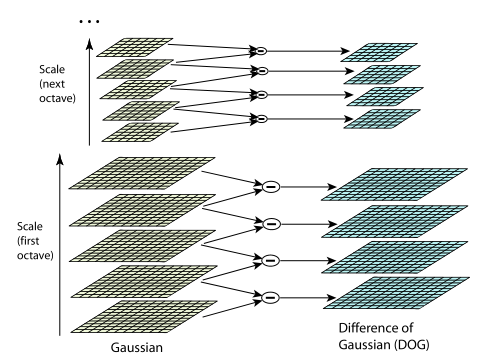
\includegraphics[width=0.6\textwidth]{dog.png}
    \caption{Пирамида Гаусианнов}
    \label{fig:dog1}
\end{figure}

После построения пирамиды разностей гауссианов по всем точкам в пирамиде ищутся локальные экстремумы. Если точка больше (меньше) всех своих 26 соседей (Рис. 2) в пирамиде разностей, то она считается ключевой.

\begin{figure}[h]
    \centering
    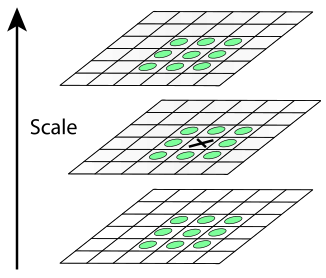
\includegraphics[width=0.5\textwidth]{dog2.png}
    \caption{Локальный экстремум в пирамиде Гауссианов}
    \label{fig:dog2}
\end{figure}

Таким образом мы для исходных изображений разных размеров мы получим ключевые точки (и небольшую область возле них) одного и того же размера - это и даёт инвариантность относительно масштабирования.

\vspace{1em}

Направление ключевой точки вычисляется исходя из направлений градиентов точек, соседних с особой. Все вычисления градиентов производятся на изображении в пирамиде гауссианов, с масштабом наиболее близким к масштабу ключевой точки. Величина и направление градиента в точке $(x,y)$ вычисляются по формулам (3) и (4) соответственно.

\begin{equation}
    m(x,y)=\sqrt{(L(x+1,y) - L(x-1,y))^2 + (L(x,y+1) - L(x,y-1))^2}
\end{equation}
\begin{equation}
    \theta(x,y)=\arctan{\left(\frac{L(x,y+1) - L(x,y-1)}{L(x+1,y) - L(x-1,y)}\right)}
\end{equation}

Направление считается в $\sigma$-окрестности ключевой точки.  Каждая точка окресности $(x, y)$ вносит вклад и итоговое значение считается за направление ключевой точки.

\subsubsection*{Извлечение дескрипторов}

\tab Как уже говорилось ранее - дескриптор должен очень хорошо и уникально описывать ключевую точку. В общем случае это может быть любой объект, который будет выполнять данные функции и являтся инвариантным относительно преобразований исходного изображения.

В алгоритме SIFT дескриптор представляет из себя вестор, содержащий информацию об окрестности ключевой точки. Дескриптор вычисляется на том же гауссиане, на котом получен оптимальный размер особой точки. Перед вычислением, для достижения инвариантности относительно поворота изображения всю область ключевой точки поворачивают на угол направления ключевой точки.

\begin{figure}[h]
    \centering
    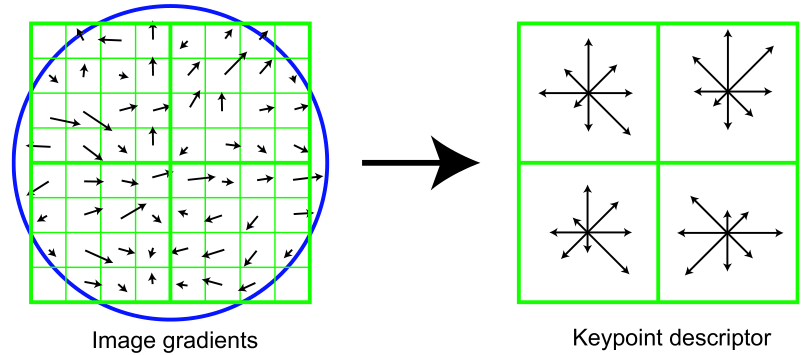
\includegraphics[width=0.8\textwidth]{desc.png}
    \caption{Получение дескриптора}
    \label{fig:desc}
\end{figure}

На Рис.3 показана окрестность ключевой точки (слева) и полученный на её основе дескриптор (справа). Маленькая стрелочка, в центре каждого пикселя в $\sigma$-окрестности обозначает градиент этого пикселя. Круг обозначает окно свертки с гауссовым ядром. Для этого ядра определяется $\sigma$, равное половине ширины окна дескриптора. В дальнейшем значение каждой точки окна дескриптора будет домножаться на значение гауссова ядра в этой точке, как на весовой коэффициент.

\vspace{1em}

Как видно справа дескриптор имеет размерность 2x2x8 (количество регионов по горизонтали, количество регионов по вертикали, количество компонент гистограммы этих регионов). Гистограма для каждого региона строится в соответствии со значениями градиентов пикселей, входящих в  $\sigma$-окрестность (8 штук):

\begin{enumerate}
    \item Каждая гистограмма так же покрывает участок в 360 градусов и делит его на 8 частей;
    \item В качестве весового коэффициента берется значение гауссова ядра, общего для всего дескриптора;
    \item В качестве ещё одних весовых коэффициентов берутся коэффициенты трилинейной интерполяции;
\end{enumerate}

Каждому градиенту в окне дескриптора можно приписать три вещественные координаты $(x, y, n)$, где $x$ — расстояние до градиента по горизонтали, $y$ — расстояние по вертикали, $n$ — расстояние до направления градиента в гистограмме (имеется ввиду соответствующая гистограмма дескриптора, в которую вносит вклад этот градиент). Коэффициент трилинейной интерполяции определяется для каждой координаты $(x, y, n)$ градиента как $1-d$, где $d$ равно расстоянию от координаты градиента до середины того единичного промежутка в который эта координата попала. Каждое вхождение градиента в гистограмму умножается на все три весовых коэффициента трилинейной интерполяции.

\vspace{1em}

Дескриптор ключевой точки состоит из всех полученных гистограмм. Как уже было сказано размерность дескриптора на рисунке $32$ компоненты (2x2x8), но на практике используются дескрипторы размерности $128$ компонент (4x4x8). Полученный дескриптор нормализуется, после чего все его компоненты, значение которых больше $0.2$, урезаются до значения $0.2$ и затем дескриптор нормализуется ещё раз. В таком виде дескрипторы готовы к использованию.

\newpage